% Frame Field Problem Setup and Minimization on a Simple Domain
% A detailed walkthrough of the mathematical formulation

\documentclass[aspectratio=169]{beamer}
\usetheme{Madrid}
\usecolortheme{default}

% Packages
\usepackage{amsmath}
\usepackage{amssymb}
\usepackage{tikz}
\usepackage{graphicx}
\usepackage{algorithm}
\usepackage{algorithmic}
\usetikzlibrary{arrows,shapes,positioning,calc}

% Custom colors
\definecolor{darkblue}{RGB}{0,51,102}
\definecolor{lightblue}{RGB}{102,153,204}
\definecolor{orange}{RGB}{255,128,0}
\definecolor{red}{RGB}{204,0,0}
\definecolor{darkred}{RGB}{153,0,0}

% Title page information
\title{Frame Field Generation}
\subtitle{Problem Setup and Minimization on a Simple Domain}
\author{Structured Grid Generation via Frame Fields}
\date{\today}

\begin{document}

% Title slide
\begin{frame}
\titlepage
\end{frame}

% Table of contents
\begin{frame}{Outline}
\tableofcontents
\end{frame}

%===============================================================================
\section{Background}
%===============================================================================

\begin{frame}{What is a Frame Field?}
\begin{columns}
\begin{column}{0.5\textwidth}
\textbf{Definition:}
\begin{itemize}
    \item A frame field assigns a cross (4 orthogonal directions) to each vertex (or face) of a mesh
    \item Rotational symmetry: directions are equivalent up to $\pm\pi/2$ rotations
    \item Used to guide quadrilateral mesh generation
\end{itemize}

\vspace{0.3cm}
\textbf{Angle Representation $\theta_i$:}
\begin{itemize}
    \item Reference edge: local coordinate system
    \item Angle $\theta_i$: rotation of frame
    \item 4 directions by rotating $\theta_i$ by $r \cdot \frac{\pi}{2}$, $r \in \{0,1,2,3\}.$ 
\end{itemize}
\end{column}

\begin{column}{0.5\textwidth}
\centering
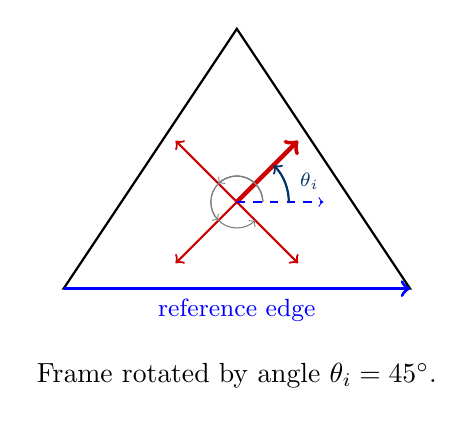
\begin{tikzpicture}[scale=2.2]
    % Triangle
    \draw[thick] (0,0) -- (2,0) -- (1,1.5) -- cycle;
    
    % Reference edge (highlighted)
    \draw[->, very thick, blue] (0,0) -- (2.0,0) node[midway, below] {\small reference edge};
    
    % Cross field at center (rotated by theta)
    \coordinate (center) at (1,0.5);
    \def\thetaA{45}
    \draw[->, ultra thick, red] (center) -- ++({0.5*cos(\thetaA)},{0.5*sin(\thetaA)});
    \draw[->, thick, red] (center) -- ++({-0.5*cos(\thetaA)},{-0.5*sin(\thetaA)});
    \draw[->, thick, red] (center) -- ++({0.5*cos(\thetaA+90)},{0.5*sin(\thetaA+90)});
    \draw[->, thick, red] (center) -- ++({-0.5*cos(\thetaA+90)},{-0.5*sin(\thetaA+90)});
    \draw[->, dashed, blue] (center) -- ++(0.5,0);
    
    % Angle arc
    \draw[->, thick, darkblue] (center) ++(0.3,0) arc (0:\thetaA:0.3);
    \node[darkblue] at ($(center)+(0.42,0.12)$) {\scriptsize $\theta_i$};

    % draw the other rotations
    \draw[->, thin, gray] (center) ++(0.15,0) arc (0:\thetaA+90:0.15);
    \draw[->, thin, gray] (center) ++(0.15,0) arc (0:\thetaA+180:0.15);
    \draw[->, thin, gray] (center) ++(0.15,0) arc (0:\thetaA+270:0.15);
    
    \node at (1,-0.5) {Frame rotated by angle $\theta_i = 45^\circ.$};
\end{tikzpicture}
\end{column}
\end{columns}
\end{frame}

\begin{frame}{Goal: Smooth Frame Field}
\begin{block}{Objective}
Find a frame field that is as \emph{smooth} as possible across the mesh, while respecting a set of user constraints.
\end{block}

\vspace{0.3cm}

\textbf{Smoothness means:}
\begin{itemize}
    \item Neighboring triangle faces $f_i$ and $f_j$ should have aligned frames
    \item Minimize rotation difference between adjacent faces 
    \item Allow for integer period jumps ($\pi/2$ rotations)
\end{itemize}

\vspace{0.3cm}

\begin{center}
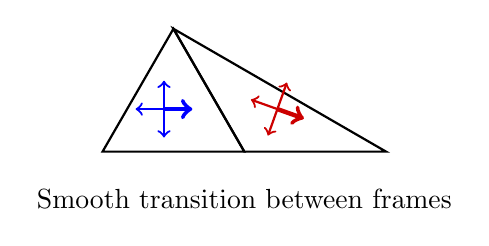
\begin{tikzpicture}[scale=1.2]
    % Two adjacent triangles
    \draw[thick] (0,0) -- (1.5,0) -- (0.75,1.3) -- cycle;
    \draw[thick] (1.5,0) -- (3,0) -- (0.75,1.3) -- cycle;
    
    % Cross field in first triangle
    \coordinate (c1) at (0.65,0.45);
    \draw[->, ultra thick, blue] (c1) -- ++(0.3,0);
    \draw[->, thick, blue] (c1) -- ++(-0.3,0);
    \draw[->, thick, blue] (c1) -- ++(0,0.3);
    \draw[->, thick, blue] (c1) -- ++(0,-0.3);
    
    % Cross field in second triangle (slightly rotated)
    \coordinate (c2) at (1.85,0.45);
    \draw[->, thick, red] (c2) -- ++(-0.28,0.1);
    \draw[->, ultra thick, red] (c2) -- ++(0.28,-0.1);
    \draw[->, thick, red] (c2) -- ++(0.1,0.28);
    \draw[->, thick, red] (c2) -- ++(-0.1,-0.28);
    
    \node[below] at (1.5,-0.3) {Smooth transition between frames};
\end{tikzpicture}
\end{center}
\end{frame}

\begin{frame}{Local $\pi/2$ Rotational Symmetry}
\begin{columns}
\begin{column}{0.55\textwidth}
\textbf{Key observation:}
\begin{itemize}
    \item Cross frames have 4-fold rotational symmetry
    \item Locally rotating by $\pi/2$ gives an equivalent frame
    \item Adjacent frames can differ by integer multiples of $\pi/2$
\end{itemize}

\vspace{0.3cm}

\textbf{Period jump $p_{ij}$:}
\begin{itemize}
    \item Integer value: $p_{ij} \in \mathbb{Z}$
    \item Represents number of $\pi/2$ rotations
    \item Allows frames to "jump" 
\end{itemize}
\end{column}

\begin{column}{0.45\textwidth}
\centering
\textbf{Examples of period jumps:}

\vspace{0.3cm}

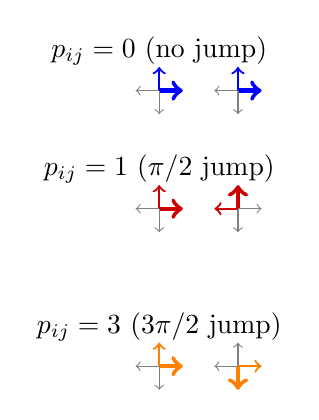
\begin{tikzpicture}[scale=1.0]
    % p = 0 case
    \node at (0,2.5) {$p_{ij} = 0$ (no jump)};
    \coordinate (c1) at (0,2);
    \draw[->, ultra thick, blue] (c1) -- ++(0.3,0);
    \draw[->, thick, blue] (c1) -- ++(0,0.3);
    \draw[->, thin, gray] (c1) -- ++ (-0.3,0);
    \draw[->, thin, gray] (c1) -- ++ (0,-0.3);
    
    \coordinate (c2) at (1,2);
    \draw[->, ultra thick, blue] (c2) -- ++(0.3,0);
    \draw[->, thick, blue] (c2) -- ++(0,0.3);
    \draw[->, thin, gray] (c2) -- ++ (-0.3,0);
    \draw[->, thin, gray] (c2) -- ++ (0,-0.3);
    
    % p = 1 case
    \node at (0,1.0) {$p_{ij} = 1$ ($\pi/2$ jump)};
    \coordinate (c3) at (0,0.5);
    \draw[->, ultra thick, red] (c3) -- ++(0.3,0);
    \draw[->, thick, red] (c3) -- ++(0,0.3);
    \draw[->, thin, gray] (c3) -- ++ (-0.3,0);
    \draw[->, thin, gray] (c3) -- ++ (0,-0.3);
    
    \coordinate (c4) at (1,0.5);
    \draw[->, ultra thick, red] (c4) -- ++(0,0.3);
    \draw[->, thick, red] (c4) -- ++(-0.3,0);
    \draw[->, thin, gray] (c4) -- ++ (0,-0.3);
    \draw[->, thin, gray] (c4) -- ++ (0.3,0);
    
    % p = -1 case
    \node at (0,-1.0) {$p_{ij} = 3$ ($3\pi/2$ jump)};
    \coordinate (c5) at (0,-1.5);
    \draw[->, ultra thick, orange] (c5) -- ++(0.3,0);
    \draw[->, thick, orange] (c5) -- ++(0,0.3);
    \draw[->, thin, gray] (c5) -- ++ (-0.3,0);
    \draw[->, thin, gray] (c5) -- ++ (0,-0.3);

    \coordinate (c6) at (1,-1.5);
    \draw[->, ultra thick, orange] (c6) -- ++(0,-0.3);
    \draw[->, thick, orange] (c6) -- ++(0.3,0);
    \draw[->, thin, gray] (c6) -- ++ (0,0.3);
    \draw[->, thin, gray] (c6) -- ++ (-0.3,0);
\end{tikzpicture}


\vspace{0.3cm}
\small
Period jumps allow frames to align while respecting $\pi/2$ symmetry
\end{column}
\end{columns}
\end{frame}


\begin{frame}{Transport Angle: $\kappa_{ij}$}
\begin{columns}
\begin{column}{0.55\textwidth}
\textbf{Definition:}
\begin{itemize}
    \item $\kappa_{ij} \in (-\pi, \pi]$ is angle between local frame of $f_i$ and $f_j$
    \item Depends only on triangle geometry (fixed)
\end{itemize}

\vspace{0.3cm}

\textbf{Computation:}
\begin{enumerate}
    \item Identify shared edge $e_{ij}$
    \item In $f_i$: compute angle $\phi_i$ between its reference edge and $e_{ij}$
    \item In $f_j$: compute angle $\phi_j$ between its reference edge and $e_{ij}$ (note orientation requires $\pi$ addition)
    \item Set $\kappa_{ij} = \phi_j - \phi_i + \pi$ (adjusted to $(-\pi, \pi]$)
\end{enumerate}

\vspace{0.3cm}

\end{column}

\begin{column}{0.45\textwidth}
\centering
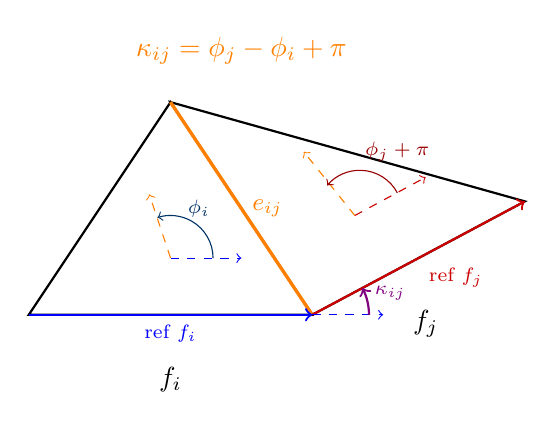
\begin{tikzpicture}[scale=1.8]
    % Two triangles sharing an edge
    \draw[thick] (0,0) -- (2,0) -- (1,1.5) -- cycle;
    \draw[thick] (2,0) -- (3.5,0.8) -- (1,1.5) -- cycle;
    
    % Shared edge (highlighted)
    \draw[very thick, orange] (2,0) -- (1,1.5) node[pos=0.5, right] {\small $e_{ij}$};
    
    % Reference edges for f_i and f_j
    \draw[->, thick, blue] (0,0) -- (2,0) node[midway, below] {\scriptsize ref $f_i$};
    \draw[->, thick, red] (2,0) -- (3.5,0.8) node[midway, below right] {\scriptsize ref $f_j$};
    
    % Angle phi_i in f_i (from reference edge to shared edge)
    \coordinate (c1) at (1,0.4);
    \draw[->, dashed, blue] (c1) -- ++(0.5,0);
    \draw[->, dashed, orange] (c1) -- ++(-0.15,0.45);
    \draw[->, thin, darkblue] (c1) ++(0.3,0) arc (0:108:0.3);
    \node[darkblue] at ($(c1)+(0.2,0.35)$) {\scriptsize $\phi_i$};
    
    % Angle phi_j in f_j (from reference edge to shared edge, note orientation)
    \coordinate (c2) at (2.3,0.7);
    \draw[->, dashed, red] (c2) -- ++(0.5,0.27);
    \draw[->, dashed, orange] (c2) -- ++(-0.36,0.45);
    \draw[->, thin, darkred] (c2) ++(0.3,0.16) arc (28:140:0.3);
    \node[darkred] at ($(c2)+(0.3,0.45)$) {\scriptsize $\phi_j + \pi$};
    
    % Kappa angle visualization (arc from ref f_i to ref f_j)
    \coordinate (base) at (2.0,0.0);
    \draw[->, dashed, blue] (base) -- ++(0.5,0);
    \draw[->, thick, violet] (base) ++(0.4,0) arc (0:28:0.4);
    \node[violet] at ($(base)+(0.55,0.15)$) {\scriptsize $\kappa_{ij}$};
    
    % Kappa formula
    \node[orange, above] at (1.5,1.7) {$\kappa_{ij} = \phi_j - \phi_i + \pi$};
    
    \node[below] at (1,-0.3) {$f_i$};
    \node[below] at (2.8,0.1) {$f_j$};
\end{tikzpicture}

\vspace{0.3cm}
\small
Transport angle $\kappa_{ij}$ is \textbf{fixed} (geometric property)
\end{column}
\end{columns}
\end{frame}



\begin{frame}{Coordinate Transformation Between Faces}
\vspace{0.1cm}

\begin{columns}
\begin{column}{0.5\textwidth}
\begin{block}{Mathematical Relationship}
For adjacent triangles $f_i$ and $f_j$, we can project $\theta_i$ into the $f_j$ local coordinate system using:
\[
    \underbrace{\theta_i}_\text{$\theta_i$ in $f_i$} \mapsto \underbrace{\theta_i + \kappa_{ij} + \frac{\pi}{2} p_{ij}}_{\theta_i \text{ in } f_j} 
\]
\end{block}

\vspace{0.3cm}

\textbf{Components:}
\begin{itemize}
    \item $\theta_i$: frame angle in $f_i$
    \item $\kappa_{ij}$: geometric rotation
    \item $\frac{\pi}{2} p_{ij}$: symmetry jump
    \item $\theta_j$: resulting angle in $f_j$
\end{itemize}
\end{column}

\begin{column}{0.5\textwidth}
\centering
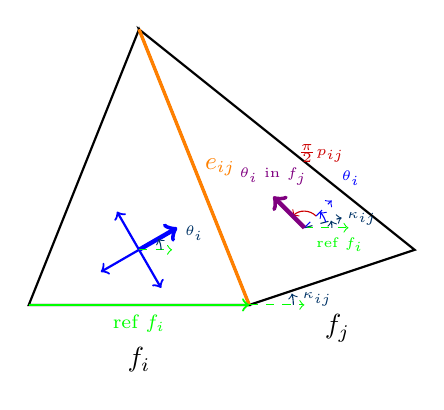
\begin{tikzpicture}[scale=1.4]
    % Two adjacent triangles
    \draw[thick] (0,0) -- (2,0) -- (1,2.5) -- cycle;
    \draw[thick] (2,0) -- (3.5,0.5) -- (1,2.5) -- cycle;
    
    % Shared edge
    \draw[very thick, orange] (2,0) -- (1,2.5) node[pos=0.5, right] {\small $e_{ij}$};
    
    % Frame in f_i with angle theta_i
    \coordinate (c1) at (1,0.5);
    \def\thetai{30}
    \draw[->, ultra thick, blue] (c1) -- ++({0.4*cos(\thetai)},{0.4*sin(\thetai)});
    \draw[->, thick, blue] (c1) -- ++({-0.4*cos(\thetai)},{-0.4*sin(\thetai)});
    \draw[->, thick, blue] (c1) -- ++({0.4*cos(\thetai+90)},{0.4*sin(\thetai+90)});
    \draw[->, thick, blue] (c1) -- ++({-0.4*cos(\thetai+90)},{-0.4*sin(\thetai+90)});
    
    % Reference direction in f_i
    \draw[->, thick, green] (0,0) -- (2,0) node[midway, below] {\scriptsize ref $f_i$};
    \draw[->, dashed, green] (c1) -- ++(0.3,0);
    \draw[->, thin, darkblue] (c1) ++(0.2,0) arc (0:\thetai:0.2);
    \node[darkblue] at ($(c1)+(0.5,0.15)$) {\tiny $\theta_i$};
    
    % Frame in f_j with angle theta_j
    % Reference direction in f_j
    \coordinate (c2) at (2.5,0.7);
    
    % \draw[->, dashed, red] (c2) -- ++(0.3,0);
    % \draw[->, thin, darkred] (c2) ++(0.2,0) arc (0:\thetaj:0.2);
    % \node[darkred] at ($(c2)+(0.35,0.2)$) {\tiny $\theta_j$};
    
    % Show the transformation step by step with arcs
    \def\kappav{15} % transport angle example
    \def\pjump{1} % period jump (0, 1, 2, or 3)
    
    % Step 1: Reference direction in f_j
    \draw[->, dashed, green] (c2) -- ++(0.4,0) node[pos=0.8, below] {\tiny ref $f_i$};
    
    % Step 2: Apply kappa_{ij} (transport angle)
    \draw[->, darkblue] (c2) ++(0.25,0) arc (0:\kappav:0.25);
    \node[darkblue, right] at ($(c2)+(0.3,0.08)$) {\tiny $\kappa_{ij}$};
    \draw[->, dashed, darkblue] (c2) -- ++({0.35*cos(\kappav)},{0.35*sin(\kappav)});
    
    % Step 3: Apply theta_i rotation
    \pgfmathsetmacro{\afterkappa}{\kappav}
    \pgfmathsetmacro{\afterthetai}{\kappav + \thetai}
    \draw[->, blue] (c2) ++({0.2*cos(\afterkappa)},{0.2*sin(\afterkappa)}) arc (\afterkappa:\afterthetai:0.2);
    \node[blue, right] at ($(c2)+(0.25,0.45)$) {\tiny $\theta_i$};
    \draw[->, dashed, blue] (c2) -- ++({0.35*cos(\afterthetai)},{0.35*sin(\afterthetai)});
    
    % Step 4: Apply period jump p_{ij} * pi/2
    \pgfmathsetmacro{\afterpjump}{\afterthetai + 90*\pjump}
    \draw[->, red] (c2) ++({0.15*cos(\afterthetai)},{0.15*sin(\afterthetai)}) arc (\afterthetai:\afterpjump:0.15);
    \node[red, above] at ($(c2)+(0.15,0.5)$) {\tiny $\frac{\pi}{2}p_{ij}$};
    
    % Final result: theta_i in f_j coordinate system
    \draw[->, ultra thick, violet] (c2) -- ++({0.4*cos(\afterpjump)},{0.4*sin(\afterpjump)}) node[above] {\tiny $\theta_i$ in $f_j$};
    
    
    \node[below] at (1,-0.3) {$f_i$};
    \node[below] at (2.8,0) {$f_j$};

    % show the kappa reference direction
    \draw[->, dashed, green] (2,0) -- ++(0.5,0);
    \draw[->, darkblue] (2,0) ++(0.4,0) arc (0:\kappav:0.4) node[midway, right] {\tiny $\kappa_{ij}$};

\end{tikzpicture}

\vspace{0.2cm}
\small
The main direction from $f_i$ (solid blue) appears in $f_j$'s coordinate system (solid purple) after applying the transformation $\theta_i + \kappa_{ij} + \frac{\pi}{2}p_{ij}$ with $p_{ij}=1$.
\end{column}
\end{columns}


\end{frame}



\begin{frame}{Smoothness Energy}
\begin{block}{Energy Definition}
The smoothness energy measures misalignment between adjacent frames:
\[
E_{\text{smooth}} = \sum_{e_{ij}} (\theta_i - \theta_j)^2 = \sum_{e_{ij}} ( \underbrace{\theta_i + \kappa_{ij} + \frac{\pi}{2} p_{ij}}_{\theta_i \text{ in } f_j} - \theta_j )^2 \overbrace{= 0}^{\text{ideal}}
\]
\end{block}

\vspace{0.3cm}

\textbf{Goal:} Minimize $E_{\text{smooth}}$ to make frames as aligned as possible with respect to user constraints.

\vspace{0.1cm}
\textbf{Difficulty:} Mixed-integer problem since $p_{ij} \in \mathbb{Z}$ (integer) and $\theta_i \in \mathbb{R}$ (continuous).


\end{frame}

%===============================================================================
\section{Optimization Problem}
%===============================================================================

\begin{frame}{Optimization Problem}
\begin{block}{Mixed Integer Problem}
For a domain with $n$ faces and $m$ period jumps, we want to solve:
\[
\min_{\vec{\theta} \in \mathbb{R}^n, \, \vec{p} \in \mathbb{Z}^m} E_{\text{smooth}}(\vec{\theta}, \vec{p}) = \min_{\vec{\theta} \in \mathbb{R}^n, \, \vec{p} \in \mathbb{Z}^m} \sum_{e_{ij}} \left( \theta_i + \kappa_{ij} + \frac{\pi}{2} p_{ij} - \theta_j \right)^2
\]
\end{block}

\vspace{0.2cm}
\textbf{Continuous relaxation:} Taking derivatives with respect to variables:

\[
    \frac{\partial E}{\partial p_{ij}} = 2\left( \theta_i + \kappa_{ij} + \frac{\pi}{2} p_{ij} - \theta_j \right) \cdot \frac{\pi}{2} = \pi\left( \theta_i + \kappa_{ij} + \frac{\pi}{2} p_{ij} - \theta_j \right) = 0
\]
\[
    \frac{\partial E}{\partial \theta_i} = \sum_{j \in N(i)} 2\left( \theta_i + \kappa_{ij} + \frac{\pi}{2} p_{ij} - \theta_j \right) = 0
\]
\end{frame}

\begin{frame}{Matrix Formulation}
\textbf{Linear system $Ax=b$ for the continuous relaxation:}
Ordering the variables as $x = (\mathbf{p}^T, \mathbf{\theta}^T)^T$:
\[  
\begin{pmatrix}
    \frac{\pi}{2} I & M^\top \\
    \frac{\pi}{2} M & L
\end{pmatrix} 
\begin{pmatrix}
    \mathbf{p} \\ \mathbf{\theta}
\end{pmatrix} = 
\begin{pmatrix}
    -\mathbf{\kappa}_{\text{edge}} \\ -\mathbf{\kappa}_{\text{vert}}
\end{pmatrix}
\]
Here, $M$ is the edge-face incidence matrix and $L = M M^\top$ is the graph Laplacian.

\vspace{0.2cm}
\footnotesize
\textbf{Explicitly for edge $k$ (connecting $i \to j$) and face $i$:}
\[
\left(
\begin{array}{ccc|ccccc}
    \ddots & 0 & 0 & & \vdots & \vdots & \\
    0 & \frac{\pi}{2} & 0 & \cdots & 1 & -1 & \cdots \\
    0 & 0 & \ddots & & \vdots & \vdots & \\
    \hline
    & \vdots & & \ddots & \vdots & \vdots & \\
    \cdots & \frac{\pi}{2} & \cdots & \cdots & \text{deg}(i) & -1 & \cdots \\
    & \vdots & & & \vdots & \ddots & 
\end{array}
\right)
\begin{pmatrix}
    \vdots \\ p_{k} \\ \vdots \\ \hline \vdots \\ \theta_i \\ \theta_j \\ \vdots
\end{pmatrix} = 
\begin{pmatrix}
    \vdots \\ -\kappa_{k} \\ \vdots \\ \hline \vdots \\ -\sum \kappa_{ij} \\ \vdots
\end{pmatrix}
\]
\end{frame}


\begin{frame}{Greedy Mixed-Integer Solver}

\begin{columns}
\begin{column}{0.55\textwidth}
\begin{algorithm}[H]
\footnotesize
\textbf{Algorithm: Greedy Rounding}
\begin{enumerate}
    \item \textbf{Initialize:} Solve continuous relaxation ($p_{ij} \in \mathbb{R}$) for global solution $x^0$.
    \item \textbf{Iterate} until all $p_{ij}$ are integers:
    \begin{itemize}
        \item Find variable $p_k$ with smallest rounding error:  $k = \arg \min_i | p_i - \text{round}(p_i) |$.
        \item \textbf{Round} and \textbf{Lock}:  $p_k \leftarrow \text{round}(p_k)$.
        \item \textbf{Update:} Re-solve for remaining free variables ($\theta, p_{\text{free}}$) to compensate for the change.
    \end{itemize}
\end{enumerate}
\end{algorithm}
\end{column}

\begin{column}{0.45\textwidth}
\small
\textbf{Why Greedy?}
\begin{itemize}
    \item \textbf{Greedy Strategy:} Rounding the "safest" variable first allows the system to \emph{relax} the remaining $\theta$ variables to compensate for the rounding error.
\end{itemize}

\vspace{0.2cm}
\textbf{Efficiency (Adaptive):}
\begin{itemize}
    \item Full re-solving is too slow.
    \item Use \textbf{Local Gauss-Seidel}: Only update variables locally dependent on the locked $p_k$.
\end{itemize}
\end{column}
\end{columns}
\end{frame}
% %===============================================================================
% \section{Simple Domain Example}
% %===============================================================================

% \begin{frame}{Simple Domain: 4 Triangles}
% \begin{columns}
% \begin{column}{0.5\textwidth}
% \textbf{Setup:}
% \begin{itemize}
%     \item Square domain: $[0,1] \times [0,1]$
%     \item Divided into 4 triangles
%     \item 5 vertices: corners + center
%     \item 6 edges (4 boundary + 2 interior)
% \end{itemize}

% \vspace{0.5cm}

% \textbf{Notation:}
% \begin{itemize}
%     \item Faces: $f_1, f_2, f_3, f_4$
%     \item Interior edges: $e_{12}, e_{23}$
%     \item Boundary edges: $e_b$
% \end{itemize}
% \end{column}

% \begin{column}{0.5\textwidth}
% \centering
% \begin{tikzpicture}[scale=3]
%     % Vertices
%     \coordinate (v1) at (0,0);
%     \coordinate (v2) at (1,0);
%     \coordinate (v3) at (1,1);
%     \coordinate (v4) at (0,1);
%     \coordinate (v5) at (0.5,0.5);
    
%     % Triangles
%     \draw[thick] (v1) -- (v2) -- (v5) -- cycle;
%     \draw[thick] (v2) -- (v3) -- (v5) -- cycle;
%     \draw[thick] (v3) -- (v4) -- (v5) -- cycle;
%     \draw[thick] (v4) -- (v1) -- (v5) -- cycle;
    
%     % Vertices labels
%     \filldraw (v1) circle (1pt) node[below left] {$v_1$};
%     \filldraw (v2) circle (1pt) node[below right] {$v_2$};
%     \filldraw (v3) circle (1pt) node[above right] {$v_3$};
%     \filldraw (v4) circle (1pt) node[above left] {$v_4$};
%     \filldraw (v5) circle (1pt) node[right] {$v_5$};
    
%     % Face labels
%     \node at (0.5,0.15) {$f_1$};
%     \node at (0.85,0.5) {$f_2$};
%     \node at (0.5,0.85) {$f_3$};
%     \node at (0.15,0.5) {$f_4$};
    
%     % Edge labels (interior)
%     \node[orange] at (0.75,0.3) {\scriptsize $e_{12}$};
%     \node[orange] at (0.75,0.7) {\scriptsize $e_{23}$};
% \end{tikzpicture}
% \end{column}
% \end{columns}
% \end{frame}

% \begin{frame}{Dual Graph Structure}
% \begin{columns}
% \begin{column}{0.5\textwidth}
% \textbf{Primal Graph (Triangulation):}
% \begin{itemize}
%     \item Vertices: $v_1, \ldots, v_5$
%     \item Edges connect vertices
%     \item Faces: triangles $f_1, \ldots, f_4$
% \end{itemize}

% \vspace{0.5cm}

% \textbf{Dual Graph:}
% \begin{itemize}
%     \item Nodes: one per triangle face
%     \item Edges: connect adjacent triangles
%     \item Edge labeled by shared primal edge
% \end{itemize}

% \vspace{0.3cm}

% $\Rightarrow$ Frame field smoothness is defined on the \textbf{dual graph}
% \end{column}

% \begin{column}{0.5\textwidth}
% \centering
% \textbf{Dual Graph:}
% \begin{tikzpicture}[scale=2.5]
%     % Dual nodes (at face centers)
%     \coordinate (d1) at (0.5,0.17);
%     \coordinate (d2) at (0.83,0.5);
%     \coordinate (d3) at (0.5,0.83);
%     \coordinate (d4) at (0.17,0.5);
    
%     % Dual edges
%     \draw[thick, blue] (d1) -- (d2);
%     \draw[thick, blue] (d2) -- (d3);
%     \draw[thick, blue] (d3) -- (d4);
%     \draw[thick, blue] (d4) -- (d1);
    
%     % Primal (light gray)
%     \draw[gray!30, thin] (0,0) -- (1,0) -- (0.5,0.5) -- cycle;
%     \draw[gray!30, thin] (1,0) -- (1,1) -- (0.5,0.5) -- cycle;
%     \draw[gray!30, thin] (1,1) -- (0,1) -- (0.5,0.5) -- cycle;
%     \draw[gray!30, thin] (0,1) -- (0,0) -- (0.5,0.5) -- cycle;
    
%     % Dual nodes
%     \filldraw[blue] (d1) circle (1.5pt) node[below] {$f_1$};
%     \filldraw[blue] (d2) circle (1.5pt) node[right] {$f_2$};
%     \filldraw[blue] (d3) circle (1.5pt) node[above] {$f_3$};
%     \filldraw[blue] (d4) circle (1.5pt) node[left] {$f_4$};
% \end{tikzpicture}

% \vspace{0.3cm}
% \small
% Dual graph: $f_1 \leftrightarrow f_2 \leftrightarrow f_3 \leftrightarrow f_4 \leftrightarrow f_1$
% \end{column}
% \end{columns}
% \end{frame}

% %===============================================================================
% \section{Mathematical Formulation}
% %===============================================================================

% \begin{frame}{Variables: Angles and Period Jumps}
% \textbf{For each triangle $f_i$:}
% \begin{itemize}
%     \item $\theta_i$ = angle of frame relative to local coordinate system
%     \item One angle per triangle: $\theta_1, \theta_2, \theta_3, \theta_4$
% \end{itemize}

% \vspace{0.5cm}

% \textbf{For each interior edge $(f_i, f_j)$:}
% \begin{itemize}
%     \item $p_{ij} \in \mathbb{Z}$ = period jump (integer multiple of $\pi/2$ rotation)
%     \item Accounts for $\pi/2$ rotational symmetry of cross
%     \item For our example: $p_{12}$ and $p_{23}$
% \end{itemize}

% \vspace{0.5cm}

% \begin{block}{Total Variables}
% In our simple domain:
% \begin{itemize}
%     \item 4 angles: $\theta_1, \theta_2, \theta_3, \theta_4$
%     \item 2 period jumps: $p_{12}, p_{23}$ (and implicitly $p_{34}, p_{41}$)
% \end{itemize}
% \end{block}
% \end{frame}


% \begin{frame}{Simple Domain Energy}
% For our 4-triangle example with interior edges $(f_1, f_2)$ and $(f_2, f_3)$:

% \begin{align*}
% E_{\text{smooth}} &= \underbrace{\left( \theta_1 + \kappa_{12} + \frac{\pi}{2} p_{12} - \theta_2 \right)^2}_{\text{edge } (f_1, f_2)} \\
% &\quad + \underbrace{\left( \theta_2 + \kappa_{23} + \frac{\pi}{2} p_{23} - \theta_3 \right)^2}_{\text{edge } (f_2, f_3)} \\
% &\quad + \underbrace{\left( \theta_3 + \kappa_{34} + \frac{\pi}{2} p_{34} - \theta_4 \right)^2}_{\text{edge } (f_3, f_4)} \\
% &\quad + \underbrace{\left( \theta_4 + \kappa_{41} + \frac{\pi}{2} p_{41} - \theta_1 \right)^2}_{\text{edge } (f_4, f_1)}
% \end{align*}

% \vspace{0.3cm}

% \textbf{Variables:}
% \begin{itemize}
%     \item Continuous: $\theta_1, \theta_2, \theta_3, \theta_4$
%     \item Integer: $p_{12}, p_{23}, p_{34}, p_{41}$
%     \item Fixed (geometry): $\kappa_{12}, \kappa_{23}, \kappa_{34}, \kappa_{41}$
% \end{itemize}
% \end{frame}

% %===============================================================================
% \section{Constraints and Topology}
% %===============================================================================

% \begin{frame}{Constraint 1: Angle Constraints}
% \textbf{User-specified angle constraints:}
% \begin{itemize}
%     \item Fix certain face angles to specific values
%     \item Example: $\theta_1 = 0$ (align frame with x-axis)
%     \item Reduces number of free variables
% \end{itemize}

% \vspace{0.3cm}

% \begin{block}{Modified Variables}
% If we constrain $\theta_1 = 0$:
% \begin{itemize}
%     \item Free angles: $\theta_2, \theta_3, \theta_4$
%     \item Constrained: $\theta_1 = 0$
% \end{itemize}
% \end{block}

% \vspace{0.3cm}

% \textbf{In the energy:}
% \begin{align*}
% E &= \left( 0 + \kappa_{12} + \frac{\pi}{2} p_{12} - \theta_2 \right)^2 + \ldots \\
% &= \left( \kappa_{12} + \frac{\pi}{2} p_{12} - \theta_2 \right)^2 + \ldots
% \end{align*}
% \end{frame}

% \begin{frame}{Constraint 2: Topological Constraints}
% \textbf{Problem:} Period jumps $p_{ij}$ must satisfy topological constraints.

% \vspace{0.3cm}

% \begin{block}{Cycle Constraint}
% Around any closed loop (cycle) in the dual graph:
% \[
% \sum_{\text{edges in cycle}} p_{ij} = 0 \pmod{4}
% \]
% \end{block}

% \vspace{0.3cm}

% \textbf{Example in our domain:}
% \begin{itemize}
%     \item Cycle: $f_1 \to f_2 \to f_3 \to f_4 \to f_1$
%     \item Constraint: $p_{12} + p_{23} + p_{34} + p_{41} \equiv 0 \pmod{4}$
%     \item This constraint comes from topology (parallel transport around loop)
% \end{itemize}

% \vspace{0.3cm}

% \textbf{Consequence:} We cannot choose all $p_{ij}$ independently!
% \end{frame}

% \begin{frame}{Spanning Tree Strategy}
% \textbf{Solution:} Use a spanning tree to eliminate cycle constraints.

% \vspace{0.3cm}

% \begin{columns}
% \begin{column}{0.5\textwidth}
% \textbf{Approach:}
% \begin{enumerate}
%     \item Compute spanning tree of dual graph
%     \item \textbf{Fix} period jumps on tree edges to zero: $p_{ij} = 0$
%     \item Keep remaining period jumps as \textbf{free variables}
% \end{enumerate}

% \vspace{0.5cm}

% \textbf{Why this works:}
% \begin{itemize}
%     \item Spanning tree has no cycles
%     \item Non-tree edges form independent cycle basis
%     \item Setting tree edges to 0 automatically satisfies all cycle constraints
% \end{itemize}
% \end{column}

% \begin{column}{0.5\textwidth}
% \centering
% \textbf{Example Spanning Tree:}
% \begin{tikzpicture}[scale=2.5]
%     % Dual nodes
%     \coordinate (d1) at (0.5,0.17);
%     \coordinate (d2) at (0.83,0.5);
%     \coordinate (d3) at (0.5,0.83);
%     \coordinate (d4) at (0.17,0.5);
    
%     % Spanning tree edges (thick red)
%     \draw[very thick, red] (d1) -- (d2);
%     \draw[very thick, red] (d2) -- (d3);
%     \draw[very thick, red] (d3) -- (d4);
    
%     % Non-tree edge (dashed blue)
%     \draw[thick, dashed, blue] (d4) -- (d1);
    
%     % Nodes
%     \filldraw (d1) circle (1.5pt) node[below] {$f_1$};
%     \filldraw (d2) circle (1.5pt) node[right] {$f_2$};
%     \filldraw (d3) circle (1.5pt) node[above] {$f_3$};
%     \filldraw (d4) circle (1.5pt) node[left] {$f_4$};
    
%     % Labels
%     \node[red, right] at (0.65,0.3) {\scriptsize $p_{12}=0$};
%     \node[red, above] at (0.7,0.65) {\scriptsize $p_{23}=0$};
%     \node[red, left] at (0.35,0.65) {\scriptsize $p_{34}=0$};
%     \node[blue, below] at (0.35,0.3) {\scriptsize $p_{41}$ free};
% \end{tikzpicture}

% \vspace{0.3cm}
% \small
% Red: tree edges ($p=0$) \\
% Blue: non-tree edge (free)
% \end{column}
% \end{columns}
% \end{frame}

% \begin{frame}{Reduced Variable Set}
% After applying spanning tree constraint:

% \vspace{0.3cm}

% \begin{block}{Variables for Optimization}
% \textbf{Fixed (constrained to zero):}
% \begin{itemize}
%     \item $p_{12} = 0, \quad p_{23} = 0, \quad p_{34} = 0$ (tree edges)
% \end{itemize}

% \textbf{Free variables:}
% \begin{itemize}
%     \item Angles: $\theta_2, \theta_3, \theta_4$ (if $\theta_1 = 0$ is constrained)
%     \item Period jump: $p_{41}$ (non-tree edge)
% \end{itemize}
% \end{block}

% \vspace{0.3cm}

% \textbf{Simplified energy:}
% \begin{align*}
% E &= \left( \kappa_{12} - \theta_2 \right)^2 \\
% &\quad + \left( \theta_2 + \kappa_{23} - \theta_3 \right)^2 \\
% &\quad + \left( \theta_3 + \kappa_{34} - \theta_4 \right)^2 \\
% &\quad + \left( \theta_4 + \kappa_{41} + \frac{\pi}{2} p_{41} \right)^2
% \end{align*}
% \end{frame}

% %===============================================================================
% \section{Minimization}
% %===============================================================================




% \begin{frame}{Stage 2: Continuous Optimization}
% Once period jumps are fixed, solve for angles.

% \vspace{0.3cm}

% \textbf{Linear system:}
% Energy is quadratic in $\theta$, so minimization gives linear equations:
% \[
% \frac{\partial E}{\partial \theta_i} = 0 \quad \text{for all free angles}
% \]

% \vspace{0.3cm}

% \textbf{For our example:}
% \begin{align*}
% \frac{\partial E}{\partial \theta_2} &= -2(\kappa_{12} - \theta_2) + 2(\theta_2 + \kappa_{23} - \theta_3) = 0 \\
% \frac{\partial E}{\partial \theta_3} &= -2(\theta_2 + \kappa_{23} - \theta_3) + 2(\theta_3 + \kappa_{34} - \theta_4) = 0 \\
% \frac{\partial E}{\partial \theta_4} &= -2(\theta_3 + \kappa_{34} - \theta_4) + 2(\theta_4 + \kappa_{41} + \frac{\pi}{2}p_{41}) = 0
% \end{align*}

% This is a $3 \times 3$ linear system: $A\theta = b$
% \end{frame}

% \begin{frame}{Matrix Form}
% \textbf{System matrix:} $A\theta = b$

% \vspace{0.3cm}

% For our example:
% \[
% \begin{bmatrix}
% 2 & -1 & 0 \\
% -1 & 2 & -1 \\
% 0 & -1 & 2
% \end{bmatrix}
% \begin{bmatrix}
% \theta_2 \\
% \theta_3 \\
% \theta_4
% \end{bmatrix}
% =
% \begin{bmatrix}
% \kappa_{12} - \kappa_{23} \\
% \kappa_{23} - \kappa_{34} \\
% \kappa_{34} - \kappa_{41} - \frac{\pi}{2}p_{41}
% \end{bmatrix}
% \]

% \vspace{0.5cm}

% \textbf{Properties:}
% \begin{itemize}
%     \item $A$ is symmetric positive definite
%     \item Sparse (tridiagonal-like for mesh topology)
%     \item Can be solved efficiently with sparse linear solvers
% \end{itemize}
% \end{frame}

% \begin{frame}{Solution Process Summary}
% \begin{enumerate}
%     \item \textbf{Preprocessing:}
%     \begin{itemize}
%         \item Load triangulation
%         \item Compute transport angles $\kappa_{ij}$ (fixed, geometry-dependent)
%         \item Build dual graph
%         \item Compute spanning tree
%         \item Apply angle constraints
%     \end{itemize}
    
%     \vspace{0.3cm}
    
%     \item \textbf{Optimization:}
%     \begin{itemize}
%         \item Initialize period jumps (tree edges: $p=0$, others: $p=0$)
%         \item \textbf{Greedy loop:}
%         \begin{enumerate}
%             \item For each free $p_{ij}$: solve linear system for $\theta$, find best integer
%             \item Update $p_{ij}$
%         \end{enumerate}
%         \item Final solve: linear system for optimal angles $\theta^*$
%     \end{itemize}
    
%     \vspace{0.3cm}
    
%     \item \textbf{Output:}
%     \begin{itemize}
%         \item Frame angle for each triangle: $\theta_i^*$
%         \item Period jumps on edges: $p_{ij}^*$
%     \end{itemize}
% \end{enumerate}
% \end{frame}

% %===============================================================================
% \section{Numerical Example}
% %===============================================================================

% \begin{frame}{Concrete Example: Square Domain}
% \textbf{Setup:}
% \begin{itemize}
%     \item 4 triangles in unit square
%     \item Assume planar (2D), so transport angles depend on edge orientations
%     \item Constrain $\theta_1 = 0$ (align with x-axis)
%     \item Use spanning tree: fix $p_{12} = p_{23} = p_{34} = 0$
% \end{itemize}

% \vspace{0.3cm}

% \textbf{Transport angles (simplified):}
% \begin{itemize}
%     \item $\kappa_{12} = 0$ (same orientation)
%     \item $\kappa_{23} = \pi/2$ (90° turn)
%     \item $\kappa_{34} = 0$
%     \item $\kappa_{41} = -\pi/2$ (back to start)
% \end{itemize}

% \vspace{0.3cm}

% \textbf{Energy:}
% \[
% E = \theta_2^2 + (\theta_2 + \pi/2 - \theta_3)^2 + (\theta_3 - \theta_4)^2 + (\theta_4 - \pi/2 + \pi p_{41}/2)^2
% \]
% \end{frame}

% \begin{frame}{Solution Steps}
% \textbf{Step 1:} Initialize $p_{41} = 0$

% \vspace{0.3cm}

% \textbf{Step 2:} Solve for angles (differentiate and set to zero):
% \begin{align*}
% 2\theta_2 + 2(\theta_2 + \pi/2 - \theta_3) &= 0 \\
% -2(\theta_2 + \pi/2 - \theta_3) + 2(\theta_3 - \theta_4) &= 0 \\
% -2(\theta_3 - \theta_4) + 2(\theta_4 - \pi/2) &= 0
% \end{align*}

% Simplifying:
% \begin{align*}
% 4\theta_2 - 2\theta_3 &= -\pi \\
% -2\theta_2 + 4\theta_3 - 2\theta_4 &= -\pi \\
% -2\theta_3 + 4\theta_4 &= \pi
% \end{align*}

% \textbf{Solution:} $\theta_2 \approx -\pi/4, \quad \theta_3 \approx 0, \quad \theta_4 \approx \pi/4$
% \end{frame}

% \begin{frame}{Visualization of Solution}
% \begin{center}
% \begin{tikzpicture}[scale=3.5]
%     % Triangulation
%     \coordinate (v1) at (0,0);
%     \coordinate (v2) at (1,0);
%     \coordinate (v3) at (1,1);
%     \coordinate (v4) at (0,1);
%     \coordinate (v5) at (0.5,0.5);
    
%     \draw[thin, gray] (v1) -- (v2) -- (v5) -- cycle;
%     \draw[thin, gray] (v2) -- (v3) -- (v5) -- cycle;
%     \draw[thin, gray] (v3) -- (v4) -- (v5) -- cycle;
%     \draw[thin, gray] (v4) -- (v1) -- (v5) -- cycle;
    
%     % Cross fields
%     \coordinate (c1) at (0.5,0.17);
%     \coordinate (c2) at (0.83,0.5);
%     \coordinate (c3) at (0.5,0.83);
%     \coordinate (c4) at (0.17,0.5);
    
%     % Frame in f1 (theta1 = 0)
%     \draw[->, very thick, red] (c1) -- ++(0.15,0);
%     \draw[->, very thick, red] (c1) -- ++(-0.15,0);
%     \draw[->, very thick, red] (c1) -- ++(0,0.15);
%     \draw[->, very thick, red] (c1) -- ++(0,-0.15);
    
%     % Frame in f2 (theta2 = -pi/4)
%     \draw[->, very thick, blue] (c2) -- ++({0.15*cos(-45)},{0.15*sin(-45)});
%     \draw[->, very thick, blue] (c2) -- ++({-0.15*cos(-45)},{-0.15*sin(-45)});
%     \draw[->, very thick, blue] (c2) -- ++({0.15*cos(45)},{0.15*sin(45)});
%     \draw[->, very thick, blue] (c2) -- ++({-0.15*cos(45)},{-0.15*sin(45)});
    
%     % Frame in f3 (theta3 = 0)
%     \draw[->, very thick, orange] (c3) -- ++(0.15,0);
%     \draw[->, very thick, orange] (c3) -- ++(-0.15,0);
%     \draw[->, very thick, orange] (c3) -- ++(0,0.15);
%     \draw[->, very thick, orange] (c3) -- ++(0,-0.15);
    
%     % Frame in f4 (theta4 = pi/4)
%     \draw[->, very thick, darkblue] (c4) -- ++({0.15*cos(45)},{0.15*sin(45)});
%     \draw[->, very thick, darkblue] (c4) -- ++({-0.15*cos(45)},{-0.15*sin(45)});
%     \draw[->, very thick, darkblue] (c4) -- ++({0.15*cos(-45)},{0.15*sin(-45)});
%     \draw[->, very thick, darkblue] (c4) -- ++({-0.15*cos(-45)},{-0.15*sin(-45)});
% \end{tikzpicture}
% \end{center}

% \vspace{0.3cm}

% \textbf{Observation:} Frames smoothly rotate around the domain, maintaining good alignment across edges.
% \end{frame}

% %===============================================================================
% \section{Conclusion}
% %===============================================================================

% \begin{frame}{Summary}
% \textbf{Problem:} Generate smooth frame field on triangulation

% \vspace{0.3cm}

% \textbf{Key components:}
% \begin{enumerate}
%     \item \textbf{Variables:} Angles $\theta_i$ per face, period jumps $p_{ij}$ per edge
%     \item \textbf{Energy:} Smoothness energy penalizes misalignment
%     \item \textbf{Constraints:}
%     \begin{itemize}
%         \item Angle constraints (user-specified)
%         \item Topological constraints (via spanning tree)
%     \end{itemize}
%     \item \textbf{Optimization:}
%     \begin{itemize}
%         \item Greedy minimization for integers $p_{ij}$
%         \item Linear solve for continuous angles $\theta_i$
%     \end{itemize}
% \end{enumerate}

% \vspace{0.3cm}

% \textbf{Result:} Frame field ready for quad mesh extraction!
% \end{frame}

% \begin{frame}{Extensions and Challenges}
% \textbf{Real-world complications:}
% \begin{itemize}
%     \item Large meshes: thousands of triangles
%     \item Curvature: transport angles non-trivial
%     \item Singularities: topological features requiring special period jumps
%     \item Hard constraints: alignment with boundary features
% \end{itemize}

% \vspace{0.3cm}

% \textbf{Advanced topics:}
% \begin{itemize}
%     \item Automatic singularity placement
%     \item Multi-resolution optimization
%     \item GPU acceleration for large problems
%     \item Integration with quad mesh extraction
% \end{itemize}

% \vspace{0.5cm}

% \begin{center}
% \Large \textbf{Thank you!}
% \end{center}
% \end{frame}

\end{document}
